
\subsection{基于流形的光滑曲面拟合问题}

\paragraph{问题描述}
基于流形方法对给定的三角剖分网格拟合光滑曲面。
% \begin{algorithm}
%   \algorithmicrequire
%   
% \end{algorithm}
\begin{description}
\item[输入] 三维空间的单纯复形面${\cal K}$(三角剖分)。
\item[输出] 同胚于$\lvert {\cal K}\rvert$,
  插值所有网格点,有四阶精度的光滑曲面$S$。
\end{description}

\paragraph{基于流形方法构造的优点}
流形把复杂的整体建模问题转化成更容易解决的局部小问题。
不同于在曲面边界上用复杂的边界条件来拼接样条曲面的方式,
基于流形的定义,我们可以在坐标邻域的每个重合区域定义混合函数,
局部调整曲面的连续性最后达到我们期望的整体的连续性条件。
坐标邻域可以重叠,
而且每个坐标邻域上的映射函数是独立的,
所以不需要复杂的附加条件来确保边界的连续性。
在坐标图册已经给定的情况下
我们甚至可以给出和原来坐标邻域重叠的新的坐标图册,
增加了我们构造曲面的灵活性。


\begin{rem}
  基于流形的定义,
  从一个拓扑流形出发,我们可以构造出坐标邻域和与之对应的一系列同胚映射。
  反之,为了构造一个光滑流形,
  我们考虑从已有的一系列“坐标邻域”和转换函数组成的
  粘合数据\cite{gallier2012parametric}中
  构造出满足流形定义的结构,
  从而得到我们希望的光滑曲面。
  考虑流形的嵌入理论。
  任意的的紧流形可以用正则开覆盖上的单位分解嵌入在欧式空间中
  (定理\ref{thm:imbedding})。
  因此,
  反之我们可以把这个开覆盖对应的坐标邻域在欧式空间中的像用单位分解的
  函数“粘合”在一起得到原来的光滑流形。
  然而在实际构造过程中,难以保证构造的转换函数是单的,
  因此我们实际构造了伪流形。
  在实际应用中,用构造的伪流形在三维空间中表示光滑曲面仍然是成功的。
\end{rem}

\subsection{构造过程}
\label{sec:gluing}

下面我们介绍从由一系列参数邻域(邻域),粘合邻域和转换函数组成的
粘合数据\cite{gallier2012parametric,},
以及形状函数和权重函数中构造光滑曲面的过程。
本节术语的严格定义和一些定理证明参见文献[PPM]
\cite{gallier2012parametric},
本节的构造函数参见[NewCon]\cite{siqueira2009new}.

从三角剖分出发,
对三角剖分的每个顶点定义一个邻域,
任意相交非空的两个邻域自然定义了两个粘合邻域,
最后在这两个粘合邻域之间定义转换函数,
得到一组粘合数据。

\begin{nota}
 $\textbf{I}=\{v\ \vert\ v\textmd{ 是 }{\cal K} \textmd{ 的一个顶点 }\}.$
\end{nota}

\begin{rem}
  光滑曲面$S$被定义为
  伪流形${\cal M}=({\cal G},\theta_u)_{u\in\mathbf{I}}$的像
  \begin{equation}
   S=\bigcup_{v\in\mathbf{I}}\theta_v(\Omega_v).
  \end{equation}
  其中${\cal G}=((\Omega_i)_{i\in \mathbf{I}},
  (\Omega_{ij})_{(i,j)\in \mathbf{I}\times \mathbf{I}},
  (\varphi_{ji})_{(i,j)\in  \mathbf{I}\times \mathbf{I} }),$
是粘合数据,$\theta_u$是参数化函数。
\end{rem}

\subsubsection{粘合数据}
\begin{defn}
  对任意顶点$v\in \mathbf{I}$, 设$m_v$是$v$的价键,
  参数邻域($p$-邻域)$\Omega_v$定义为集合,
  \begin{equation}
     \Omega_v=\left\{(x,y)\in\mathbb{R}^2\vert x^2+y^2
    <\left(\cos\left(\frac{\pi}{m_v}\right)\right)^2\right\}.
  \end{equation}
\end{defn}


\begin{defn}
    对任意两个顶点$u$, $w\in\mathbf{I}$
    使得 $[u,w]$ 是 ${\cal K}$的一个面,
    定义函数
    \begin{displaymath}
      g_{uv}:C_u-\{(0,0)\}\rightarrow C_v-\{(0,0)\}
    \end{displaymath}
   为如下的复合函数形式
    \begin{displaymath}
       g_{uv}(p)=R^{-1}_{(v,u)}\circ g_v^{-1}\circ h
      \circ g_u\circ R_{(u,v)}(p),
    \end{displaymath}
    其中 $C_u$ 是 $P$-多项式 $P_u$的内切圆;
    $p=(r\cos\theta,r\sin\theta),r\neq 0$;
    \begin{equation}
    g_u(p)=\left(\frac{\cos(\pi/6)}{\cos(\pi/m_u)}r\cos(m_u\theta/6),
    \frac{\cos(\pi/6)}{\cos(\pi/m_u)}r\sin(m_u\theta/6)\right);
\end{equation}
\begin{equation}
     g_v^{-1}(p)=\left(\frac{\cos(\pi/m_v)}
      {\cos(\pi/6)}r\cos(6/m_v\theta),
    \frac{\cos(\pi/m_v)}{\cos(\pi/6)}r\sin(6/m_v\theta)\right);
\end{equation}
\begin{equation}
   h(p)=(1-r\cos\theta,-r\sin\theta);
\end{equation}
\begin{equation}
  R_{(u,v)}(p)=\left(r\cos\left(\theta-\frac{2\pi i}{m_u}\right),
    r\sin\left(\theta-\frac{2\pi i}{m_u}\right)\right);\quad
  R^{-1}_{(v,u)}(p)=\left(r\cos\left(\theta+\frac{2\pi j}{m_v}\right),
  r\sin\left(\theta+\frac{2\pi j}{m_v}\right)\right).
\end{equation}
    % $R_{(u,v)}(p)=e^{-\frac{2\pi i}{jm_u}}p$,
    % $R_{(v,u)}(p)=e^{-\frac{2\pi i}{lm_v}}p$,
    % and $s_u(v)=u'_j,s_v(u)=v'_l$.
  \end{defn}
\begin{figure}[H]
    \centering
    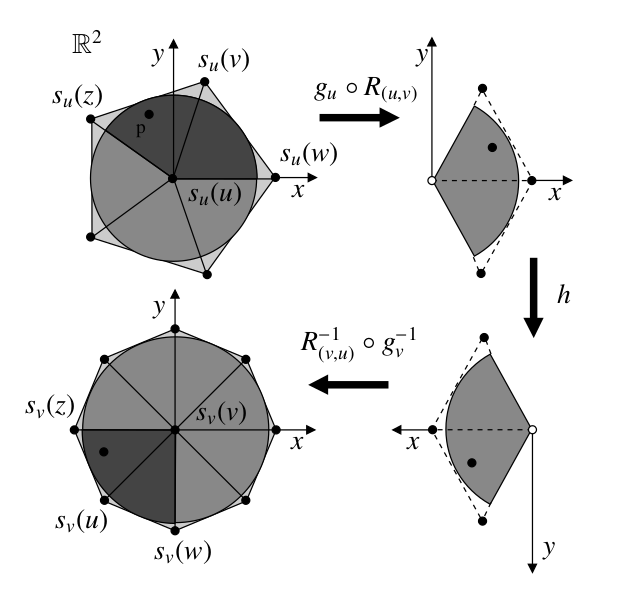
\includegraphics[width=0.3\linewidth]{fig/transferSector}
    \label{fig:sector}
  \end{figure}
  \begin{rem}
    $g_{uv}$把$C_u$的扇形区域$A$映到$C_v$的扇形区域$B$。
     $R_{(u,v)}$ 是绕着$(0,0)$的旋转。
  \end{rem}
  
  \begin{defn}[粘合邻域]
    对任意的 $u,v\in \mathbf{I},$
    \textbf{粘合邻域} $\Omega_{uv}$ 定义为
    \begin{equation*}
      \Omega_{uv}=
      \begin{cases}
        \Omega_u&\textmd{ if }$u=v$,\\
        g_{vu}(\Omega_v)\cap \Omega_u &\textmd{ 若 }
        [u,v]\textmd{ 是 }{\cal K}\textmd{ 的面 }\\
        \emptyset&\textmd{ 其他.}
      \end{cases}
    \end{equation*}
  \end{defn}
  \begin{rem}
    定义光滑微分同胚的
    转换函数$\varphi_{vu}:\Omega_{uv}\rightarrow\Omega_{vu}$.
  \end{rem}
  \begin{defn}[转换函数]
    对任意点对$(u,v)\in \mathbf{I}\times \mathbf{I}$使得
    $\Omega_{uv}\neq \emptyset$,
    \textbf{转换函数}$\varphi_{vu}:\Omega_{uv}\rightarrow\Omega_{vu}$,
    定义为
\begin{equation*}
  \forall p\in \Omega_{uv},\quad \varphi_{vu}(p)=
  \begin{cases}
    g_{uv}(p) & u\neq v\\
    p & \textmd{其他}.
  \end{cases}
\end{equation*}
  \end{defn}

\begin{rem}
  参数邻域概念对应2-流形中坐标邻域$(U,\varphi)$中的平面开集$\varphi(U)$.
\end{rem}
\begin{defn}
  粘合数据 ${\cal G}=((\Omega_i)_{i\in \mathbf{I}},
  (\Omega_{ij})_{(i,j)\in \mathbf{I}\times \mathbf{I}},
  (\varphi_{ji})_{(i,j)\in  \mathbf{I}\times \mathbf{I} })$.
\end{defn}

\subsubsection{参数化函数(参数化子)}
\label{sec:parametrizations}

\begin{defn}[权重函数]
  对$\forall u\in \mathbf{I}$,
  定义和$p$-邻域$\Omega_U$有关的\textbf{权重函数}
  $\gamma_u:\mathbb{R}^2\rightarrow\mathbb{R}$如下:
  \begin{equation}
      \gamma_u(p)=\xi(\sqrt{x^2+y^2}),
  \end{equation}
其中
\begin{equation}
  \xi(t)=
    \begin{cases}
      1 &t\leq 0.25\cos(\pi/m_u)\\
      0&t\geq \cos(\pi/m_u)\\
      1/(1+e^{2\cdot l}) &\textmd{otherwise}
    \end{cases};
    \quad
    l=\left(\frac{1}{\sqrt{1-H}}\right)-\left(\frac{1}{\sqrt{H}}\right);
    \quad 
  H=\left(\frac{t- 0.25\cos(\pi/m_u)}{ 0.75\cos(\pi/m_u)}\right).
\end{equation}
\end{defn}
\begin{rem}
  $\gamma_u$在紧支集$\Omega_u$上大于0,且$\gamma_u$是解析函数。
  $\gamma_u$的光滑性保证了最后构造的曲面的光滑性。
\end{rem}

\begin{rem}
  所有的$p$-邻域$\Omega_u$组成的集合$\mathscr{D}$对应流形上开覆盖的概念,
  $\{\gamma_u\}$对应紧支集在开覆盖的开集中的函数。
\end{rem}
\begin{rem}
  用最小二乘拟合Bézier曲面片来定义形状函数。
  由于形状函数定义在每个点$u$的局部邻域$\Omega_u$,
  我们需要先用三角剖分的顶点拟合一个近似原来三角剖分的曲面$S'$.
  如果$S'$的拟合精度有四阶,用$S'$上在点$u$附近的点拟合最小二乘曲面
  的误差精度也可能有四阶。(需要测试)
  这里我们采用PN三角曲面片(参见章节\ref{sec:PNTriangle})
  构造$S'$,
  PN三角曲面片的精度需要测试。
\end{rem}

\begin{defn}
  \label{defn:shape}
  对任意$u\in \mathbf{I}$,
  $\Omega_u$上的\textbf{形状函数}
  $\psi_u:\mathbb{R}^2\rightarrow \mathbb{R}^3,$
  定义为$(m,n)$次的张量Bézier曲面片:
  \begin{equation}
    \label{eq:Bézier}
    \psi_u(p)=\sum_{0\leq j\leq m}\sum_{0\leq k\leq n}
    b^u_{j,k}\cdot B_j^m(x)\cdot B_k^n(y),
  \end{equation}
  其中$(x,y)$是关于关于仿射结构$[-L,L]\times [-L,L]$的坐标,
  且$L=\cos(\pi/m_u)$;
  $\{b_{j,k}^u\subset \mathbb{R}^3\}$是Bézier曲面片控制点;
  $B^l_i(t)=\binom{l}{i}\left(\frac{r-t}{r-s}\right)^{l-i}
  \left(\frac{t-s}{r-s}\right)^{i}$
  是关于仿射结构$[s-r]$的第$i$个$l$次Bernstein多项式,
  $i\in \{0,1,\ldots,l\}$.
  取$\psi_u$的次数$(m,u)$为$(m_u+1,m_u+1)$.
\end{defn}

\begin{figure}[H]
    \centering
    \includegraphics[width=0.3\linewidth]{fig/shape}
    \label{fig:shape}
  \end{figure}

\begin{defn}
  对任意的顶点 $u\in \mathbf{I},$
  定义在参数邻域$\Omega_u$上的\textbf{参数化子}
  $\theta_u:\Omega_u\rightarrow \theta_u(\Omega_u)\subset\mathbb{R}^3$,
  在任意点$p\in \Omega_u$定义为
  \begin{displaymath}
    \theta_u(p)=\sum_{v\in J_u(p)}\omega_{vu}(p)\times (\psi_v\circ
    \varphi_{vu}(p)),
  \end{displaymath}
其中
\begin{equation}
  \omega_{vu}(p)=\frac{\gamma_v\circ\varphi_{vu}(p)}
  {\sum_{w\in J_u(p)}\gamma_w\circ\varphi_{wu}(p)},\quad
  J_u(p)=\{v\vert p\in \Omega_{uv}\}\subset I.
\end{equation}
\end{defn}

\begin{rem}
  $\omega_{vu}$的概念对应于从属于开覆盖的单位分解
  (见定义\ref{defn:unitDecompose})。
\end{rem}
\subsection{算法}



